% Copyright (C) 2007 Technical University of Liberec.  All rights reserved.
%
% Please make a following refer to Flow123d on your project site if you use the program for any purpose,
% especially for academic research:
% Flow123d, Research Centre: Advanced Remedial Technologies, Technical University of Liberec, Czech Republic
%
% This program is free software; you can redistribute it and/or modify it under the terms
% of the GNU General Public License version 3 as published by the Free Software Foundation.
%
% This program is distributed in the hope that it will be useful, but WITHOUT ANY WARRANTY;
% without even the implied warranty of MERCHANTABILITY or FITNESS FOR A PARTICULAR PURPOSE.
% See the GNU General Public License for more details.
%
% You should have received a copy of the GNU General Public License along with this program; if not,
% write to the Free Software Foundation, Inc., 59 Temple Place - Suite 330, Boston, MA 021110-1307, USA.
%
%
%
% use PDFLatex to compile this
%


In this chapter we are comparing the computing efficiency of released versions of Flow123d. We provide some 
of the time profiling information gathered from benchmarks, point out and discuss the differences umong different 
versions.

We use the class \verb'Profiler' to get time profiling information -- measured times that are taken by running different 
pieces of code. Selected problems are solved with different versions and different number 
of processors is used in parallel computation also to see scaling efficiency.

Two consecutively released versions 1.6.7 and 1.7.0 has been profiled so far. 
Benchmarks are computed on cluster 'hal' in the Supercomputing Centre of Czech Technical University.


\section{Problem of transport in Melechov region}

\begin{table}[!htb]
\centering
\begin{tabular}{ll}
date & June 6, 2013 \\
mesh size & 56355 elements \\
compared versions & 1.6.7 (rev. 2392) flow123d/branches/1.6.7 \\
                  & 1.7.0 (rev. 2416) flow123d/trunk \\
data available on Bacula server & pavel.exner/flow123d\_benchmarks
\end{tabular}
\caption{Benchmark general information}
\label{tab:bench1}
\end{table}

This benchmark is based on the real data. We are solving transport of a single 
substance from the concentration source in the Melechov region which is considered as
one of the localities suitable for building nuclear waste deposit. The results of profiling can be seen in
the table \ref{tab:profiler_Mel1}. One can see in the header of the table that the problem was computed several times on different 
number of proccessors, with both versions 1.6.7 and 1.7.0. Number of calls of different routines and 
maximum amount of time which is spent on one of the proccessors during the routine (column \emph{Tmax}) have been measured.
We will now discuss some of the results which are highlighted in \ref{tab:profiler_Mel1}.


\begin{itemize}
\item \textbf{Assembly.} The amount of time needed for \emph{assembly} of the mixed hybrid system (in \emph{Darcy constructor}) 
was mainly increased by moving some of the precomputations from mesh reading routines directly into the assembly proccess. 
This is the part which we can optimize in the future and futhermore we would like to make it faster by implementing numerical 
integration using new system of classes for handling degrees of freedom, finite element values etc.

\item \textbf{Mesh reading.} Another thing that is slowing down the computation is reading of the mesh. Version 1.7.0 seems 
to be slower because the neighboring of elements is computed directly in runtime. By contrast the older version uses still 
the utility 'NGH' to generete neighboring file which is used later (this procedure is not measured). We can also see along the 
row \emph{Reading mesh} that this routine is not scaling at all. Until we implement classes for handling the mesh in parallel 
way this will not be any faster.

\item \textbf{Solving MH System.} We can see the increase in time needed for solving mixed hybrid system. The computation 
of Schur complements needs to be optimized.

\item \textbf{Convection matrix assembly.}
In the \emph{convection matrix assembly} routine we can see improvement from version 1.6.7 to 1.7.0. This routine scales better in
newer version and this probably can be still further optimized.

\item \textbf{Transport Operator Splitting -- one step.}
It seems the newer version 1.7.0 is a bit faster. The difference is mainly caused by some small changes in determining the time step of convection. 
There are fewer convection steps in version 1.7.0 so the routine does not last so long. But still the average time of one convection step 
is shorter.

\item \textbf{Output.} There are two parts of the output -- output of the Darcy flow computation (row \emph{Darcy output}) and 
output of the transport operator splitting method (row \emph{TOS-output}). We can see that both have been slowed down 
(output of water flow almost twice) and that both of them are not scaling at all. The problem of
slowing down is currently being solved. Next step will be taken in making the code parallel as soon as we have parallel mesh available.

\end{itemize}

\pagebreak

\clearpage

\begin{sidewaystable}[!htbp]
\scriptsize
\begin{tabular}{|l|r|r|r|r|r|r|r|r|r|r|r|r|r|r|r|r|}
\hline
proccessors                            & \multicolumn{4}{c|}{1} & \multicolumn{4}{c|}{2} & \multicolumn{4}{c|}{4} & \multicolumn{4}{c|}{8} \\
\hline
version                                & \multicolumn{2}{c|}{1.6.7} & \multicolumn{2}{c|}{1.7.0} &  \multicolumn{2}{c|}{1.6.7} & \multicolumn{2}{c|}{1.7.0} &   \multicolumn{2}{c|}{1.6.7} & \multicolumn{2}{c|}{1.7.0} & \multicolumn{2}{c|}{1.6.7} & \multicolumn{2}{c|}{1.7.0}  \\
\hline
measurement                            & calls &  Tmax  & calls  &  Tmax  & calls  &  Tmax  & calls  &  Tmax  & calls  &  Tmax  & calls  &  Tmax  & calls  &  Tmax  & calls  &  Tmax  \\
\hline
Whole Program                          &   1   &   98.23   &   1   &   86.92   &   1   &   31.17   &   1   &   35.48   &   1   &   21.58   &   1   &   26.42   &   1   &   18.39   &   1   &   23.67   \\
 HC run simulation                     &   1   &   92.83   &   1   &   79.05   &   1   &   25.87   &   1   &   29.3    &   1   &   16.36   &   1   &   20.51   &   1   &   13.25   &   1   &   17.84   \\
  convection matrix assembly           &   1   &   0.16    &   1   &   0.25    &   1   &   1.32    &   1   &   0.1 &   1   &   1.31    &   1   &   0.07    &   1   &   1.3 &   1   &   0.06    \\
  TOS-output data                      &   5   &   2.3 &   5   &   2.45    &   5   &   2.31    &   5   &   2.59    &   5   &   2.32    &   5   &   2.55    &   5   &   2.32    &   5   &   2.54    \\
  Solving MH system                    &   1   &   4.29    &   1   &   5.19    &   1   &   1.95    &   1   &   2.97    &   1   &   1.06    &   1   &   1.7 &   1   &   0.73    &   1   &   1.28    \\
   solve system                      &   1   &   3.05    &   1   &   2.52    &   1   &   1.02    &   1   &   1.02    &   1   &   0.57    &   1   &   0.57    &   1   &   0.38    &   1   &   0.43    \\
    iteration-PETSC solver         &   12  &   3.05    &   20  &   2.52    &   12  &   1.02    &   13  &   1.01    &   12  &   0.56    &   12  &   0.57    &   12  &   0.38    &   12  &   0.42    \\
   Schur 1                           &   1   &   0.9 &   1   &   2.14    &   1   &   0.67    &   1   &   1.46    &   1   &   0.36    &   1   &   0.84    &   1   &   0.26    &   1   &   0.63    \\
    schur1 - create,inverse         &   1   &   0.17    &   1   &   1.46    &   1   &   0.07    &   1   &   0.4 &   1   &   0.05    &   1   &   0.22    &   1   &   0.04    &   1   &   0.15    \\
    schur1 - form                   &   1   &   0.73    &   1   &   0.69    &   1   &   0.6 &   1   &   1.06    &   1   &   0.31    &   1   &   0.63    &   1   &   0.22    &   1   &   0.48    \\
   Schur 2                            &   1   &   0.33    &   1   &   0.32    &   1   &   0.25    &   1   &   0.44    &   1   &   0.14    &   1   &   0.26    &   1   &   0.1 &   1   &   0.21    \\
  TOS-one step                        &   5   &   82.64   &   5   &   64.04   &   5   &   17.66   &   5   &   15.97   &   5   &   9.14    &   5   &   8.56    &   5   &   6.37    &   5   &   6.36    \\
   convection-one step               &   16050   &   82.59   &   13790   &   64  &   16050   &   17.66   &   13790   &   15.97   &   16050   &   9.13    &   13790   &   8.55    &   16050   &   6.36    &   13790   &   6.36    \\
    mat mult                        &   16050   &   39.16   &   13790   &   26.02   &   16050   &   10.66   &   13790   &   9.05    &   16050   &   5.75    &   13790   &   4.67    &   16050   &   4.15    &   13790   &   3.29    \\
    data reinit                     &           &           &   13790   &   1.66    &           &           &   13790   &   1.05    &           &           &   13790   &   1.05    &           &           &   13790   &   1.13    \\
    compute concentration sources   &   16050   &   43.31   &   13790   &   36.25   &   16050   &   7.31    &   13790   &   6.99    &   16050   &   3.6 &   13790   &   3.03    &   16050   &   2.52    &   13790   &   2.22    \\
  Darcy output                         &   2   &   3.28    &   2   &   6.99    &   2   &   3.31    &   2   &   7.14    &   2   &   3.32    &   2   &   7.12    &   2   &   3.32    &   2   &   7.12    \\
 HC constructor                         &   1   &   5.35    &   1   &   7.79    &   1   &   5.16    &   1   &   6.32    &   1   &   5.05    &   1   &   6.05    &   1   &   5.04    &   1   &   5.99    \\
  Darcy constructor                   &   1   &   2   &   1   &   3.28    &   1   &   1.61    &   1   &   1.74    &   1   &   1.5 &   1   &   1.45    &   1   &   1.48    &   1   &   1.41    \\
   preallocation                     &   1   &   0.45    &   1   &   0.55    &   1   &   0.13    &   1   &   0.15    &   1   &   0.08    &   1   &   0.09    &   1   &   0.06    &   1   &   0.07    \\
   data init                         &       &           &   1   &   0.32    &       &           &   1   &   0.32    &       &           &   1   &   0.32    &       &           &   1   &   0.32    \\
   prepare parallel                  &   1   &   0.41    &   1   &   0.35    &   1   &   0.58    &   1   &   0.62    &   1   &   0.6 &   1   &   0.65    &   1   &   0.61    &   1   &   0.71    \\
   precalculation in mesh            &   1   &   0.5     &       &           &   1   &   0.62    &       &           &   1   &   0.62    &   &           &   1   &   0.62    &       &      \\
   assembly                          &   1   &   0.57    &   1   &   2.01    &   1   &   0.2 &   1   &   0.56    &   1   &   0.12    &   1   &   0.3 &   1   &   0.09    &   1   &   0.22    \\
  Reading mesh                        &   1   &   2.27    &   1   &   3.94    &   1   &   2.47    &   1   &   3.94    &   1   &   2.48    &   1   &   3.95    &   1   &   2.5 &   1   &   3.93    \\
   MESH - setup topology             &   1   &   1.71    &   1   &   0.49    &   1   &   1.9 &   1   &   0.49    &   1   &   1.91    &   1   &   0.49    &   1   &   1.92    &   1   &   0.5 \\
  GMSHReader - read mesh            &   1   &   0.51    &   1   &   3.46    &   1   &   0.51    &   1   &   3.45    &   1   &   0.51    &   1   &   3.46    &   1   &   0.51    &   1   &   3.43    \\
\hline
\end{tabular}
\caption{Benchmark results on the transport problem in Melechov region.}
\label{tab:profiler_Mel1}
\end{sidewaystable}

\clearpage

\section{Transport sources}
The problem of transport sources can be viewed in different ways. We can prescribe a~source term in a~region of a~mesh 
or we can cut off that region from the mesh and then prescribe a~Dirichlet boundary condition on the created boundary. 
The second way was used in some models when transport sources had not been implemented in Flow123d yet.
In this section we would like to show the user the comparision of both techniques used on the real problem.

\textbf{Water flow.} One of the problems of prescribing the Dirichlet boundary condition instead of source term that arises
is not knowing the values of pressure (or velocity) to prescribe. There is a solution for this at the moment as Flow123d provides
functionality for interpolating values between meshes. 

\begin{figure}[!h]
        \centering
        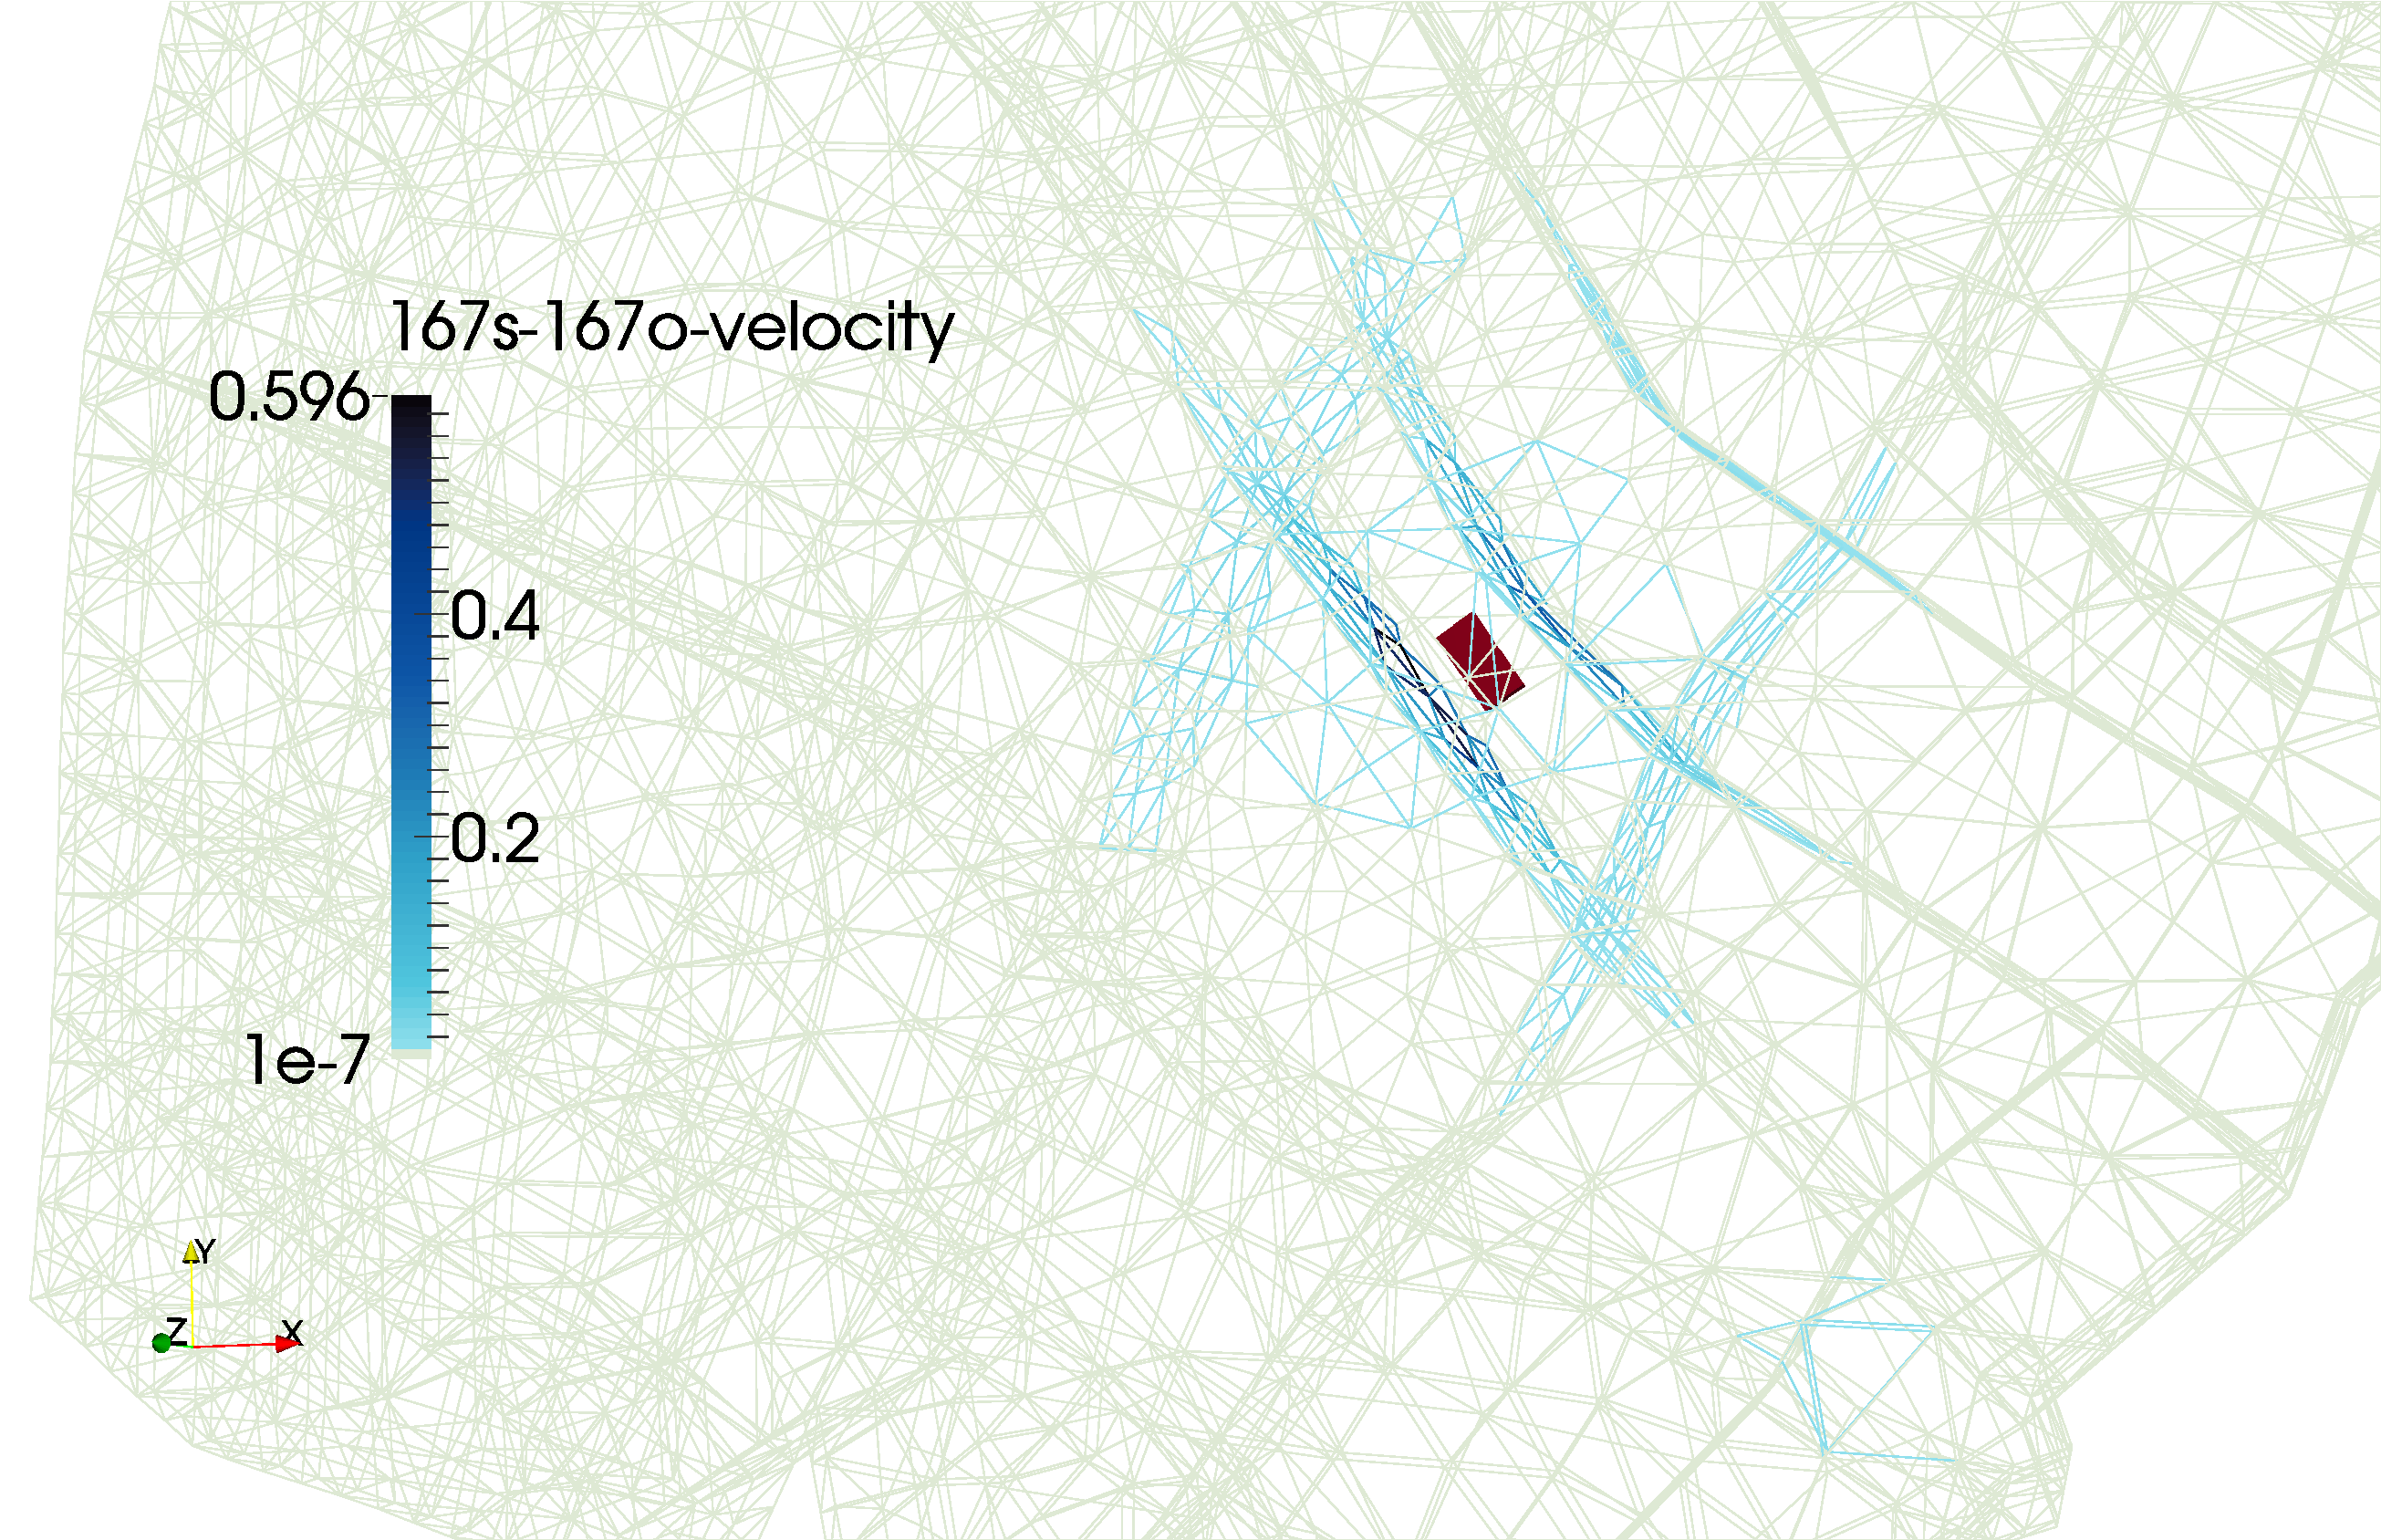
\includegraphics[width=0.55\textwidth]{tests_graphics/mel_167s-167_velocity.pdf}
        \caption{Difference in flow velocities between computation with Dirichlet BC and sources term (both computed in version 1.6.7). 
                 Red brick is the source region.}
        \label{fig:bench_mel1}
\end{figure}
%
\begin{figure}[!h]
        \centering
        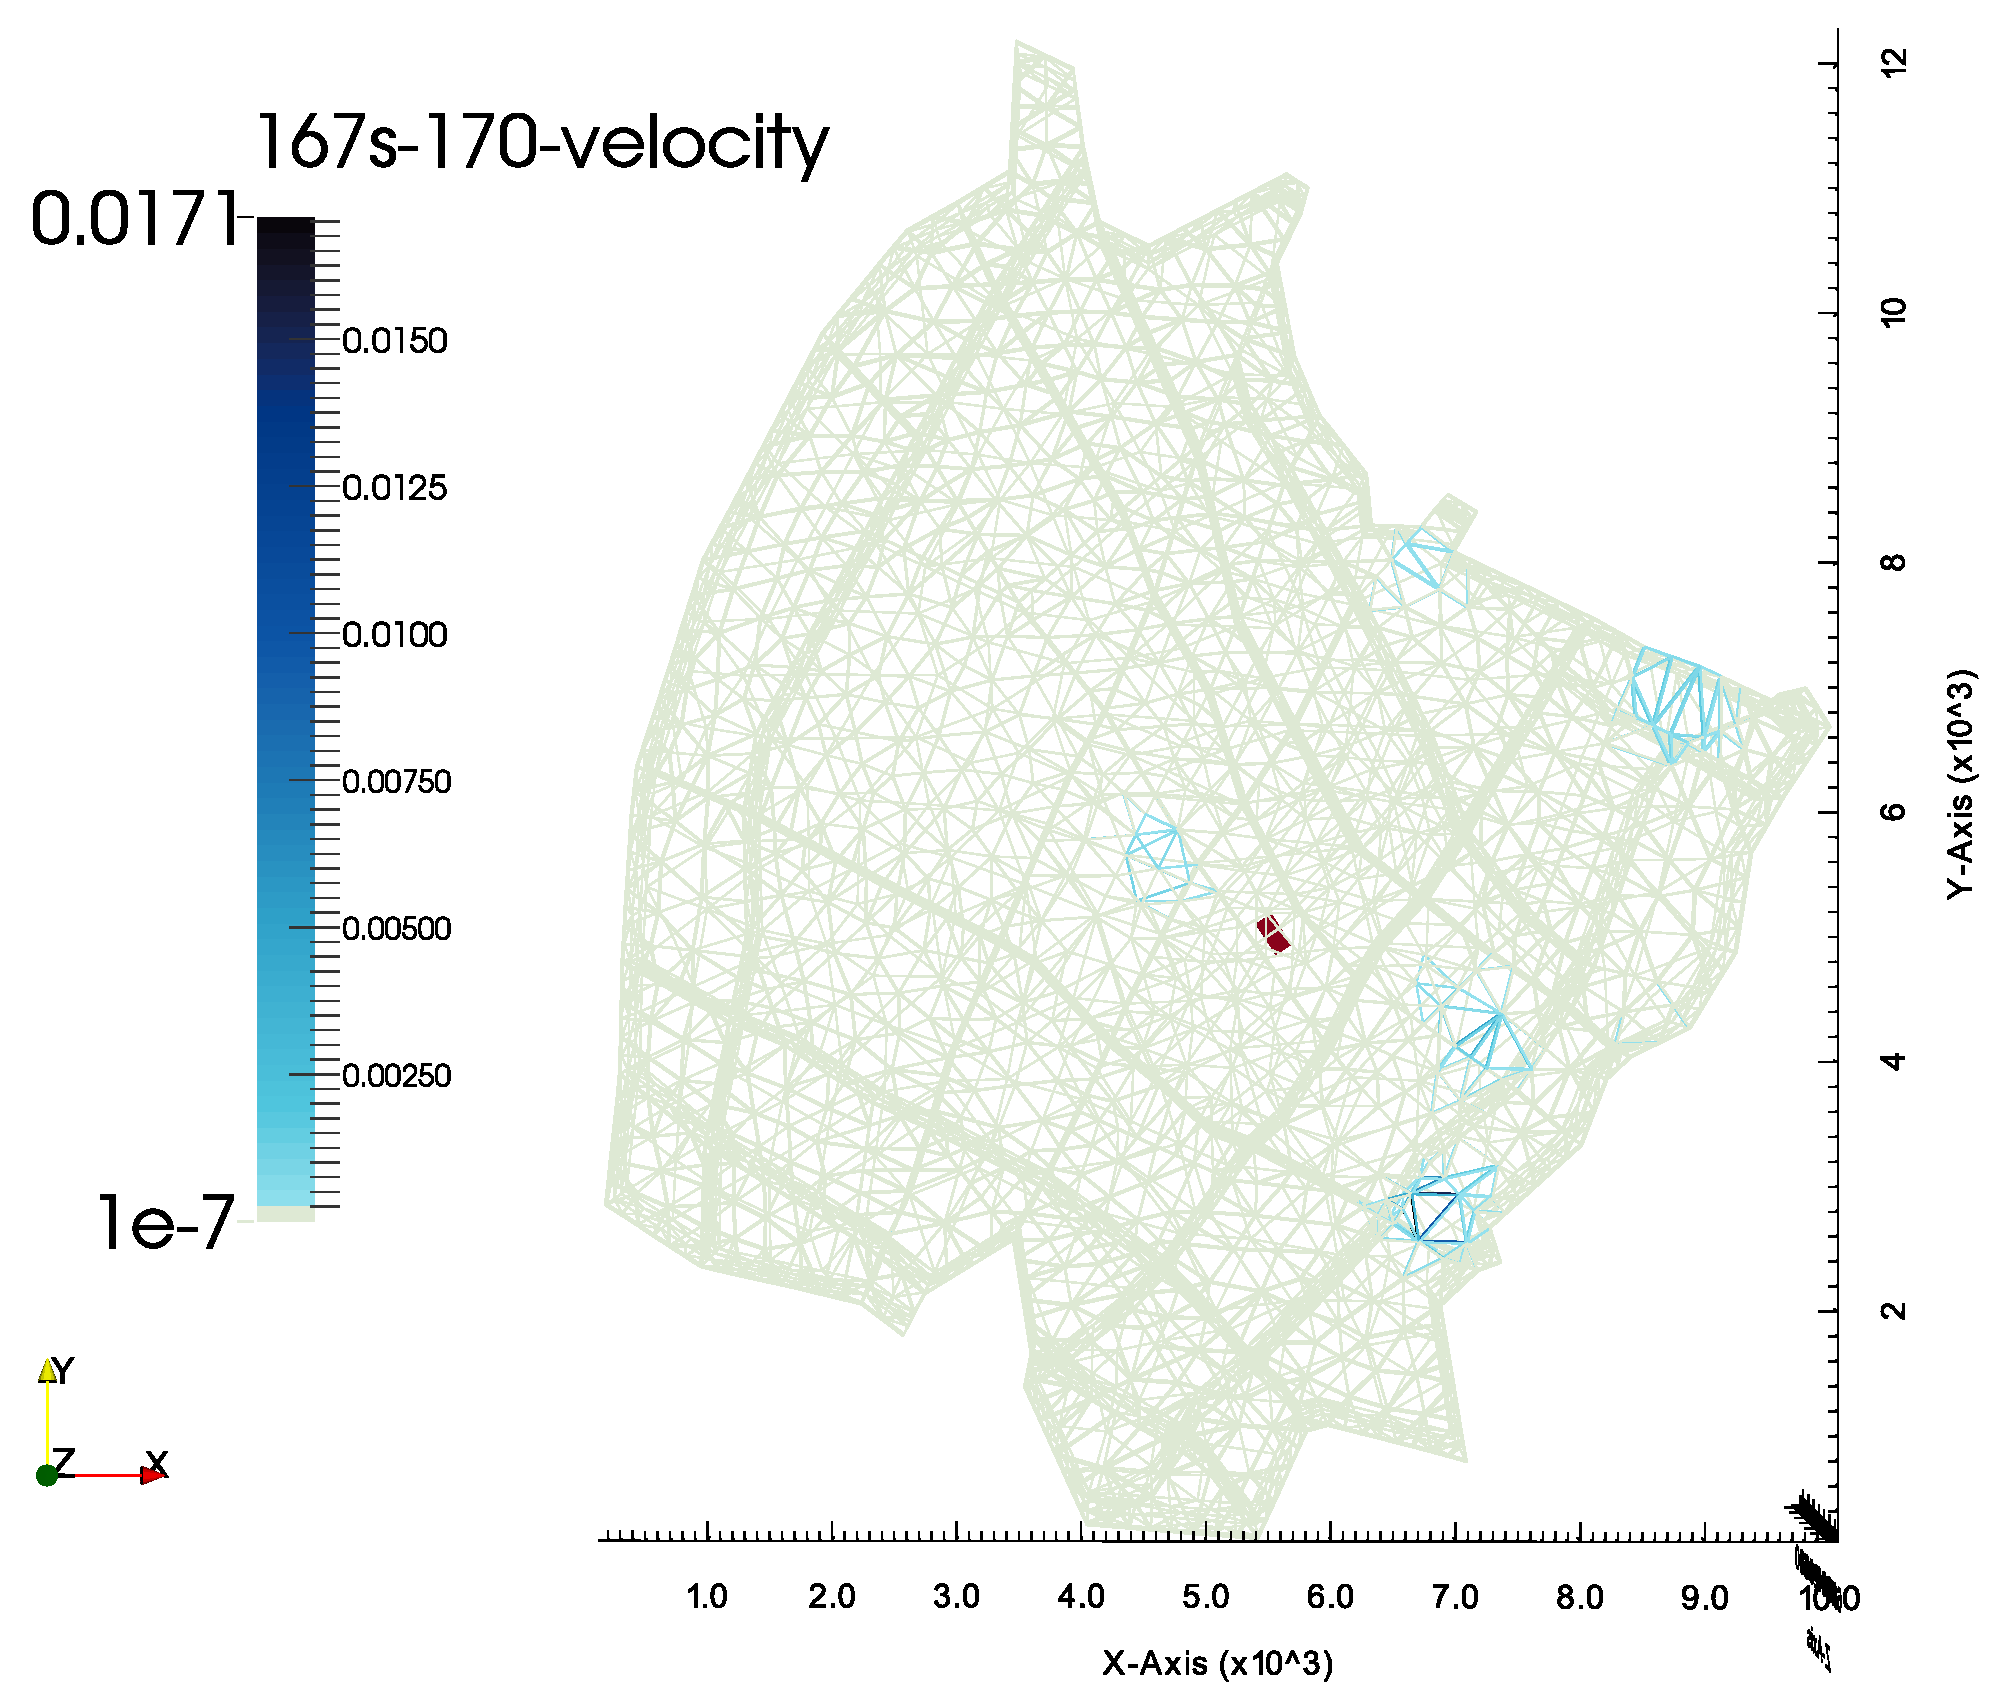
\includegraphics[width=0.65\textwidth]{tests_graphics/mel_167s-170_velocity.pdf}
        \caption{Difference in flow velocities between solutions computed by versions 1.6.7 and 1.7.0 (with sources term).
                 Red brick is the source region.}
        \label{fig:bench_mel2}
\end{figure}

In the figure \ref{fig:bench_mel1} we are showing the difference between the older solution (with Dirichlet BC prescribed on the source region) and 
solution computed with source term prescribed. We can see that there is considerable difference in the nearby area of the source. The solutions in farther 
regions is considered equal with the precision of the solver $10^{-7}$.


% \begin{figure}
%     \centering
%     \begin{subfigure}[b]{0.48\textwidth}
%         \centering
%         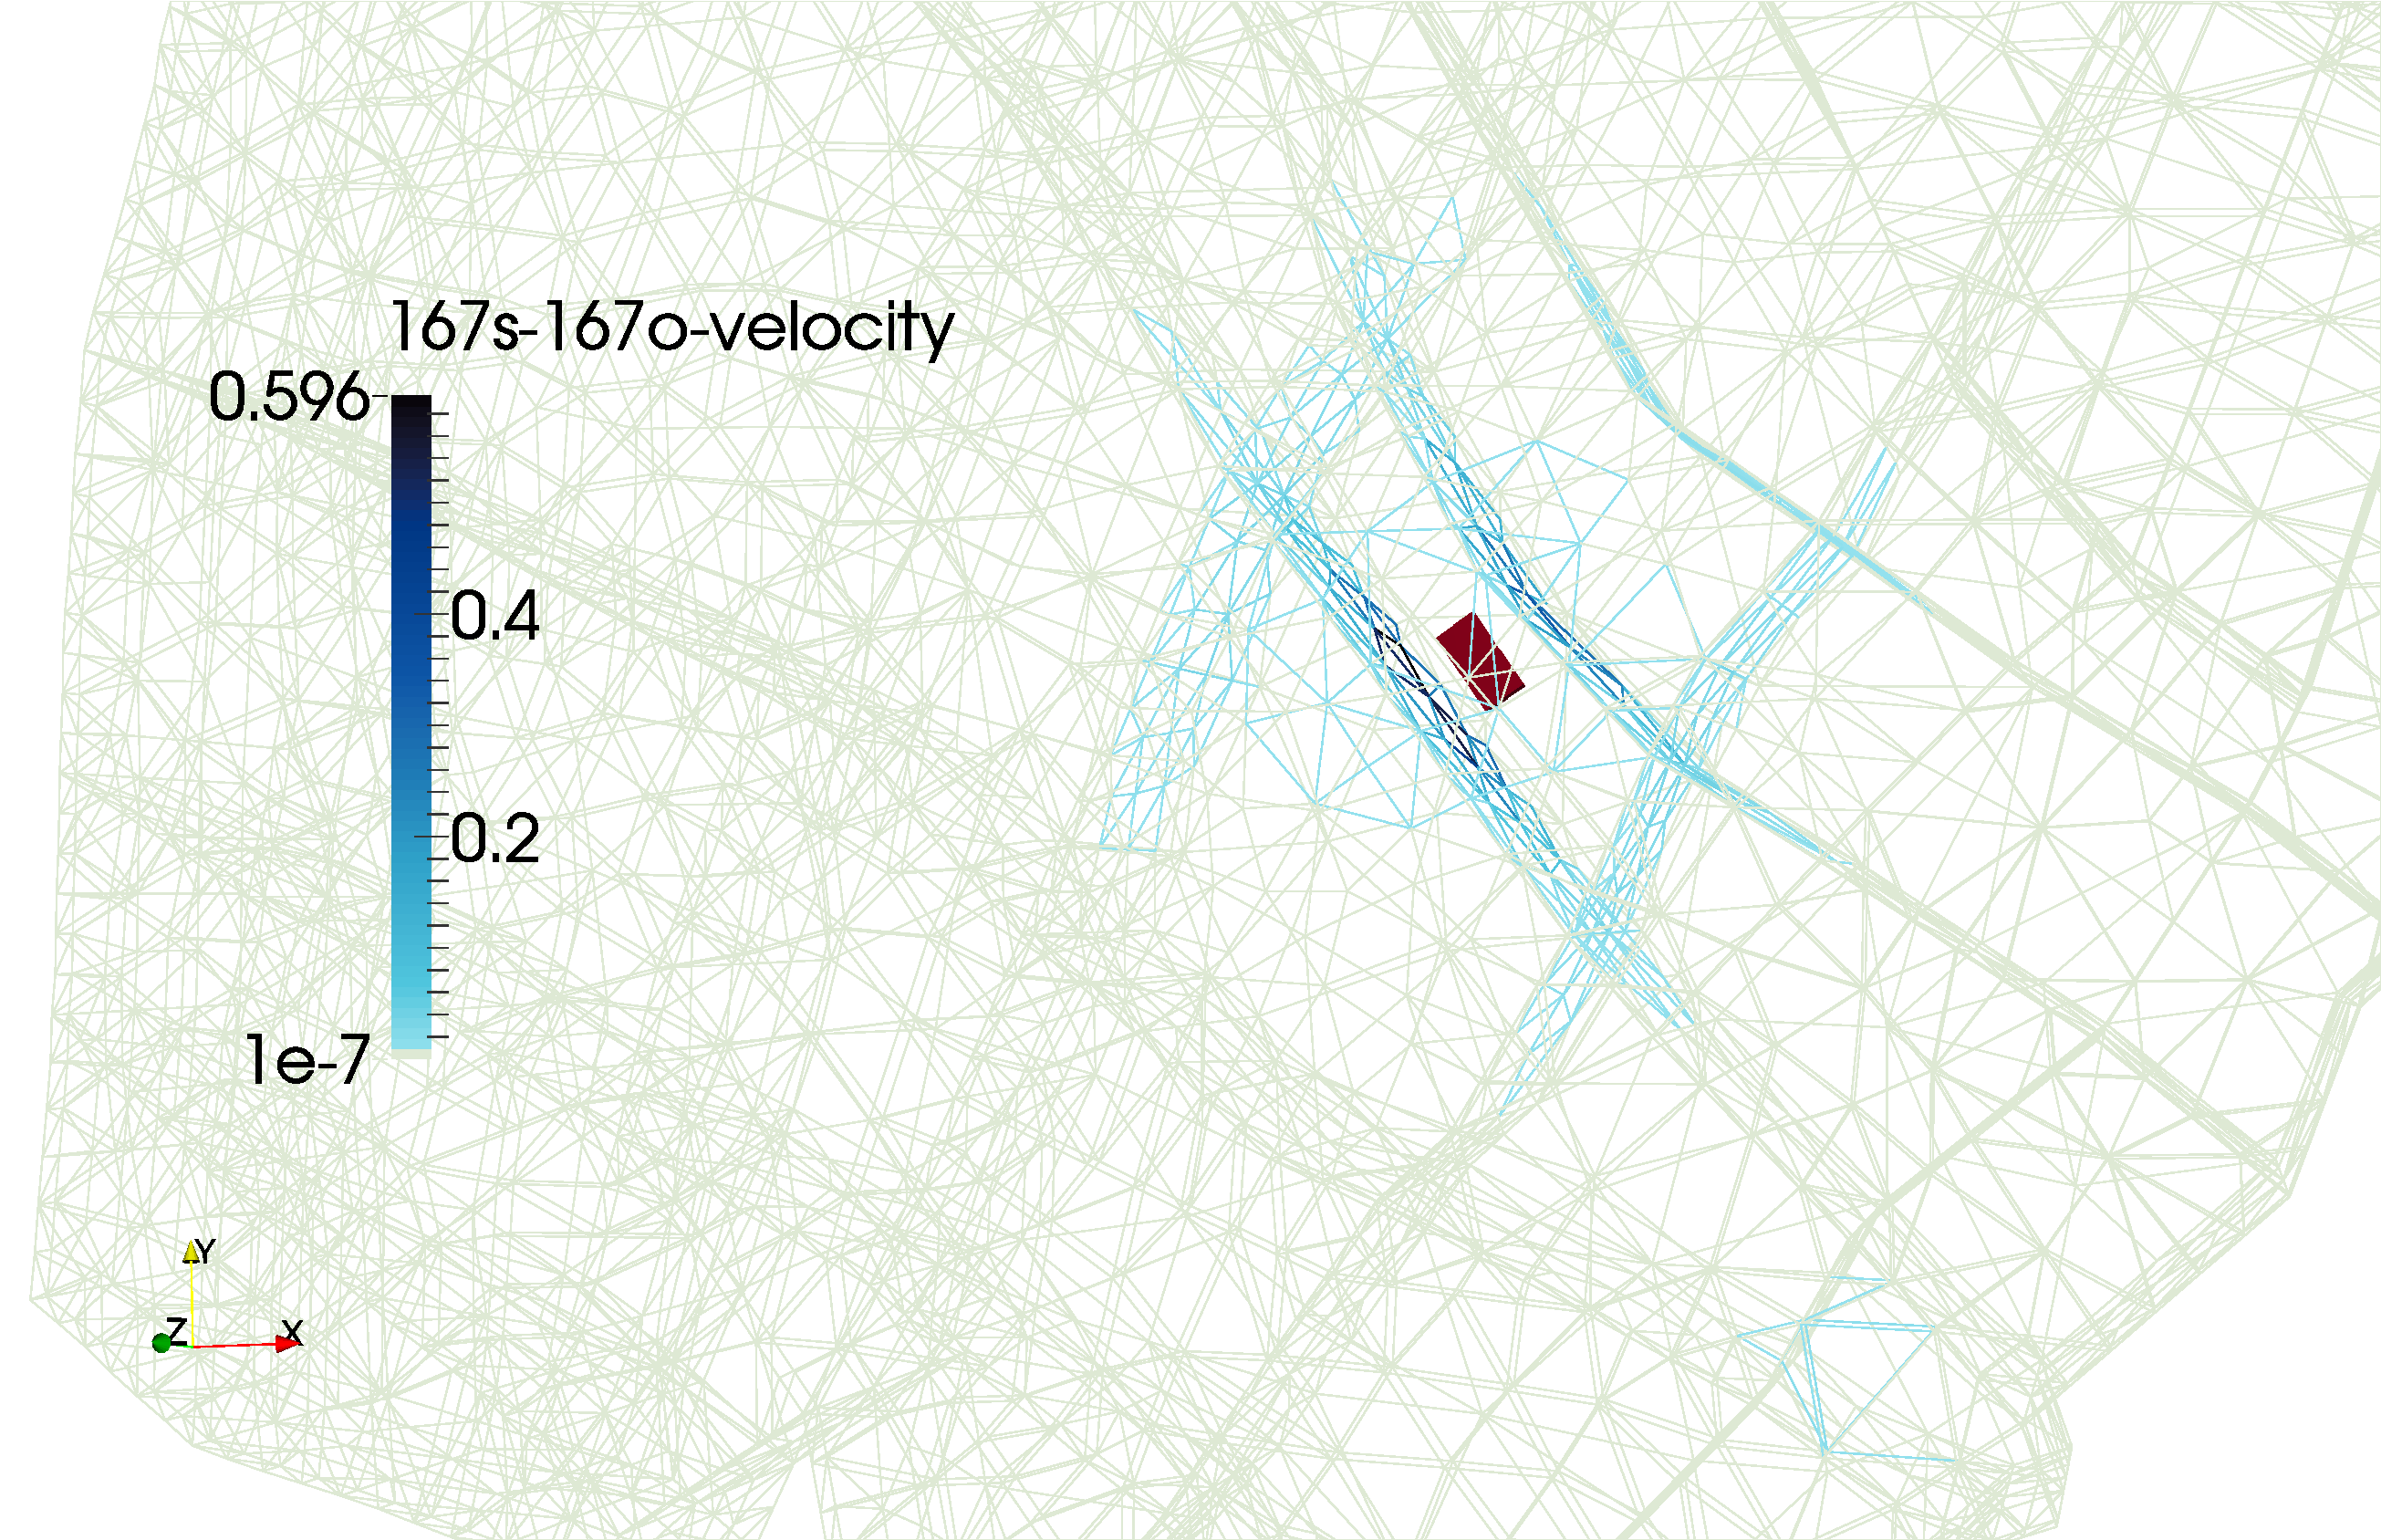
\includegraphics[width=\textwidth]{tests_graphics/mel_167s-167_velocity.pdf}
%         \caption{Elementwise pressure head and velocity field (triangles).}
%         \label{fig:bench_mel1}
%     \end{subfigure}
%     \begin{subfigure}[b]{0.48\textwidth}
%         \centering
%         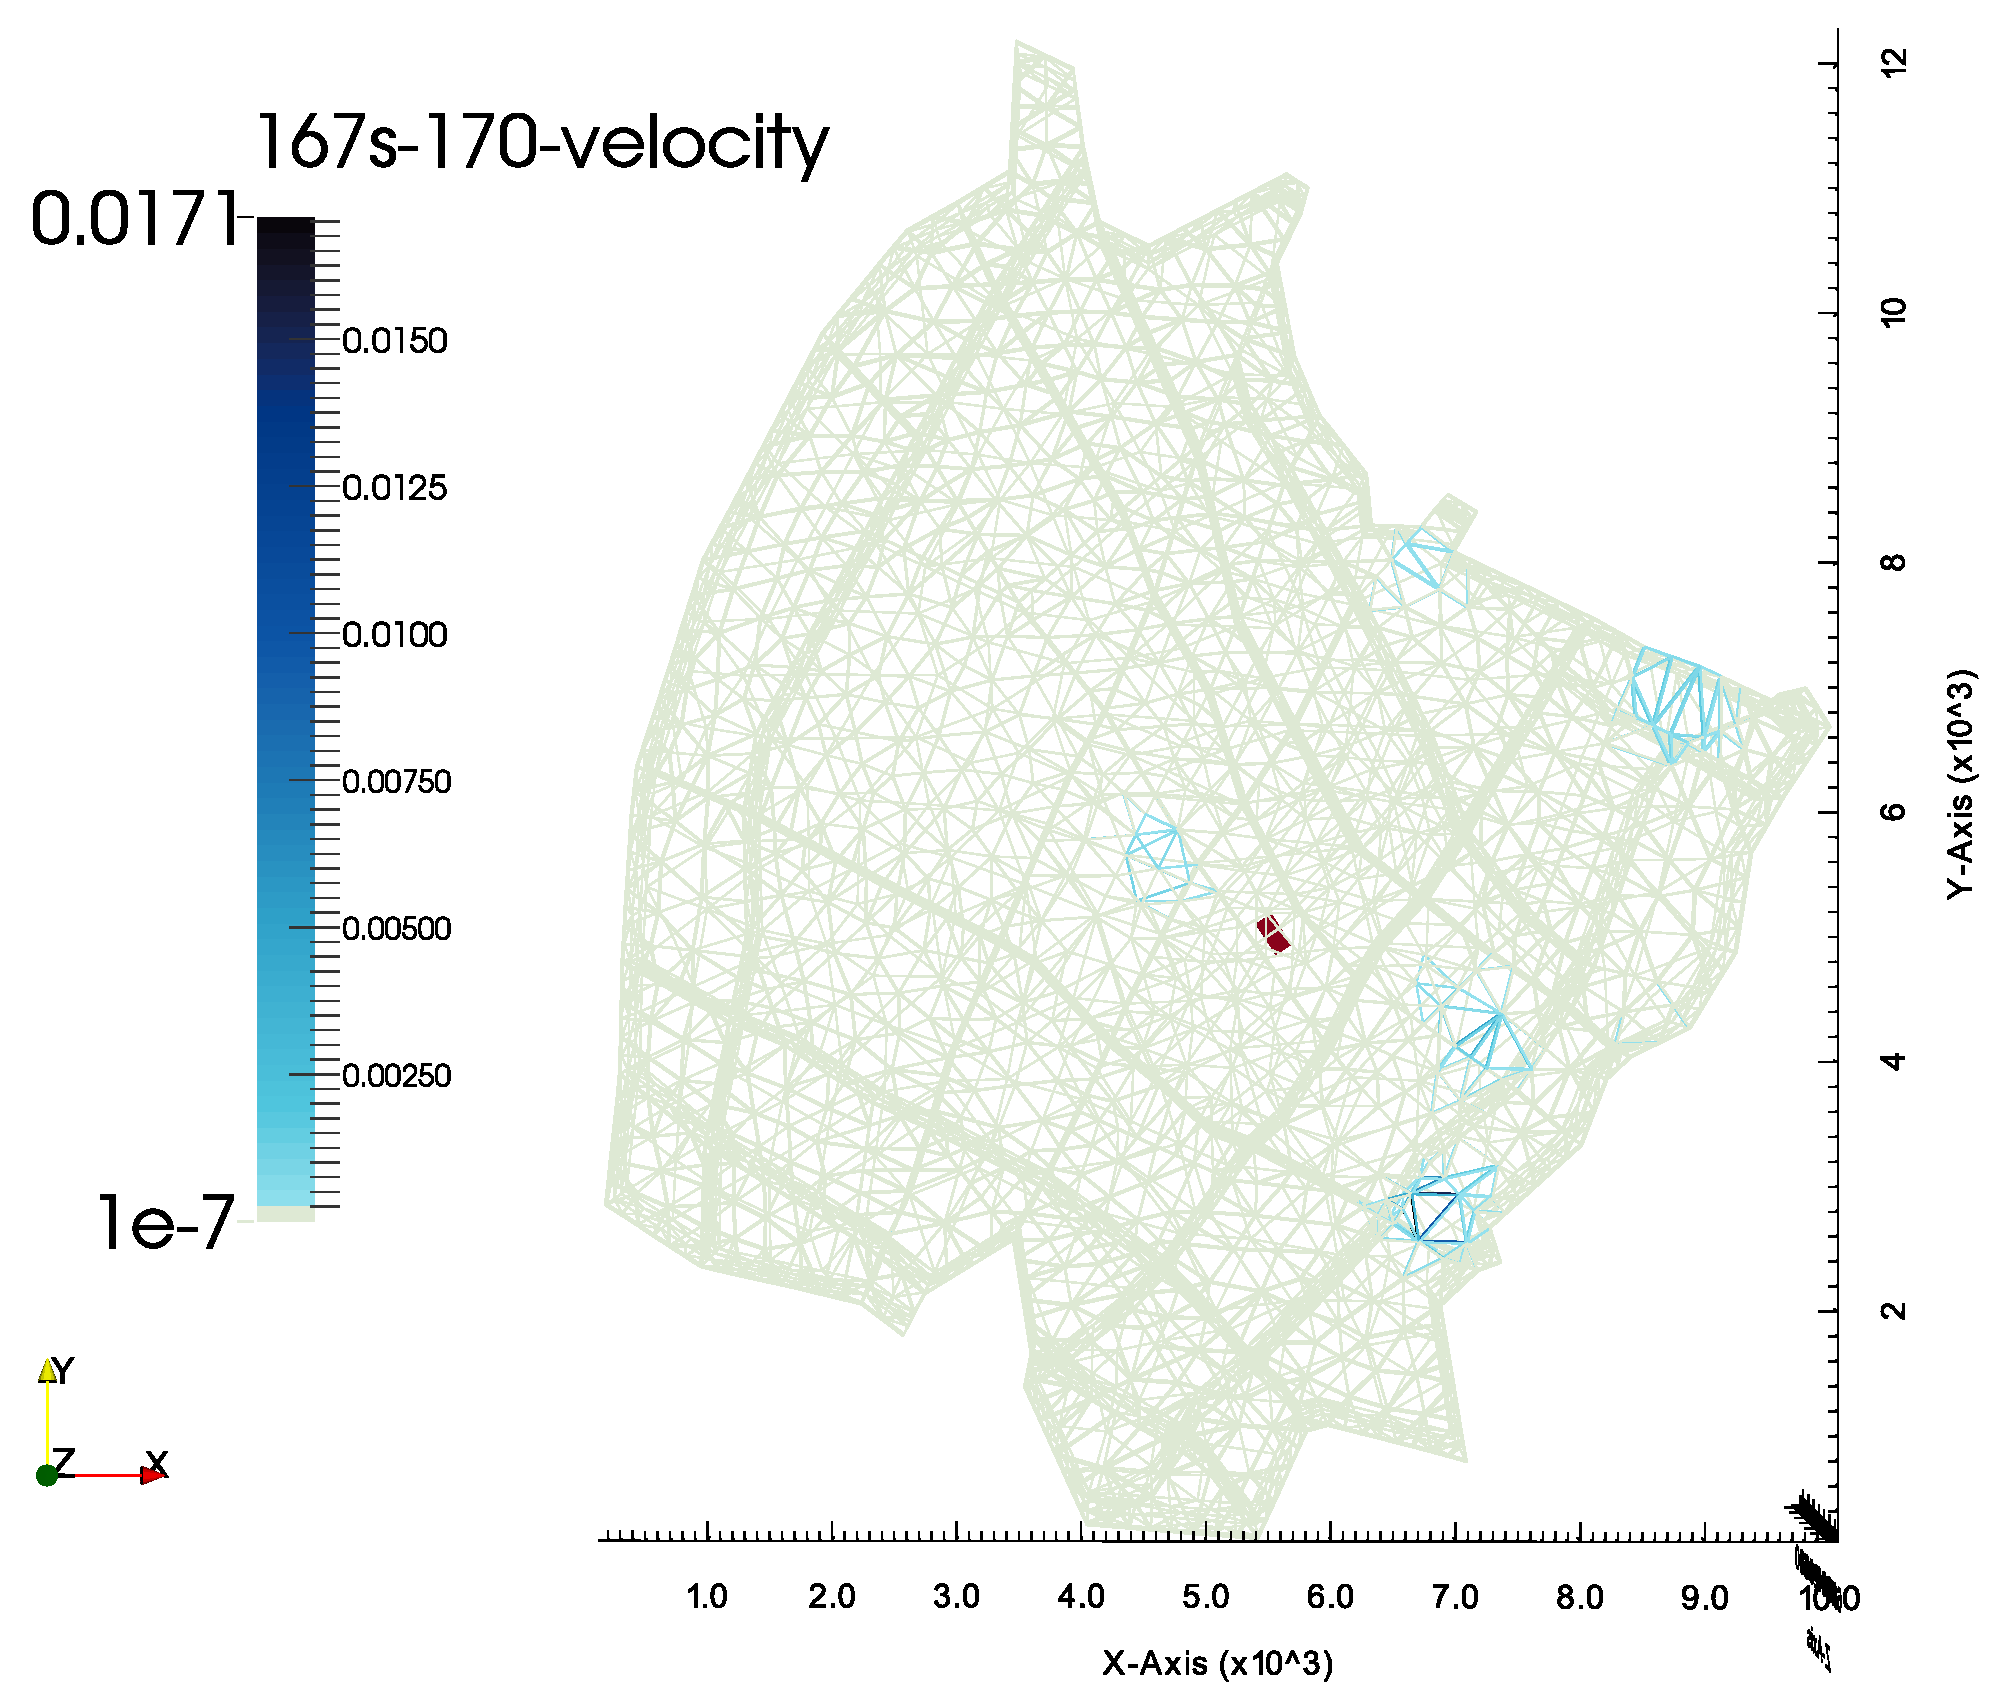
\includegraphics[width=\textwidth]{tests_graphics/mel_167s-170_velocity.pdf}
%         \caption{Elementwise pressure head and velocity field (triangles).}
%         \label{fig:bench_mel2}
%     \end{subfigure}
% \end{figure}

In the figure \ref{fig:bench_mel2} we also demonstrate small difference in water flow computed by versions 1.6.7 and 1.7.0. 
There are 5 areas where the difference if larger than the solver accuracy (set $10^{-7}$). Source of this difference 
is not clear at the moment.

\begin{figure}[!h]
    \centering
    \begin{subfigure}[b]{0.3\textwidth}
        \centering
        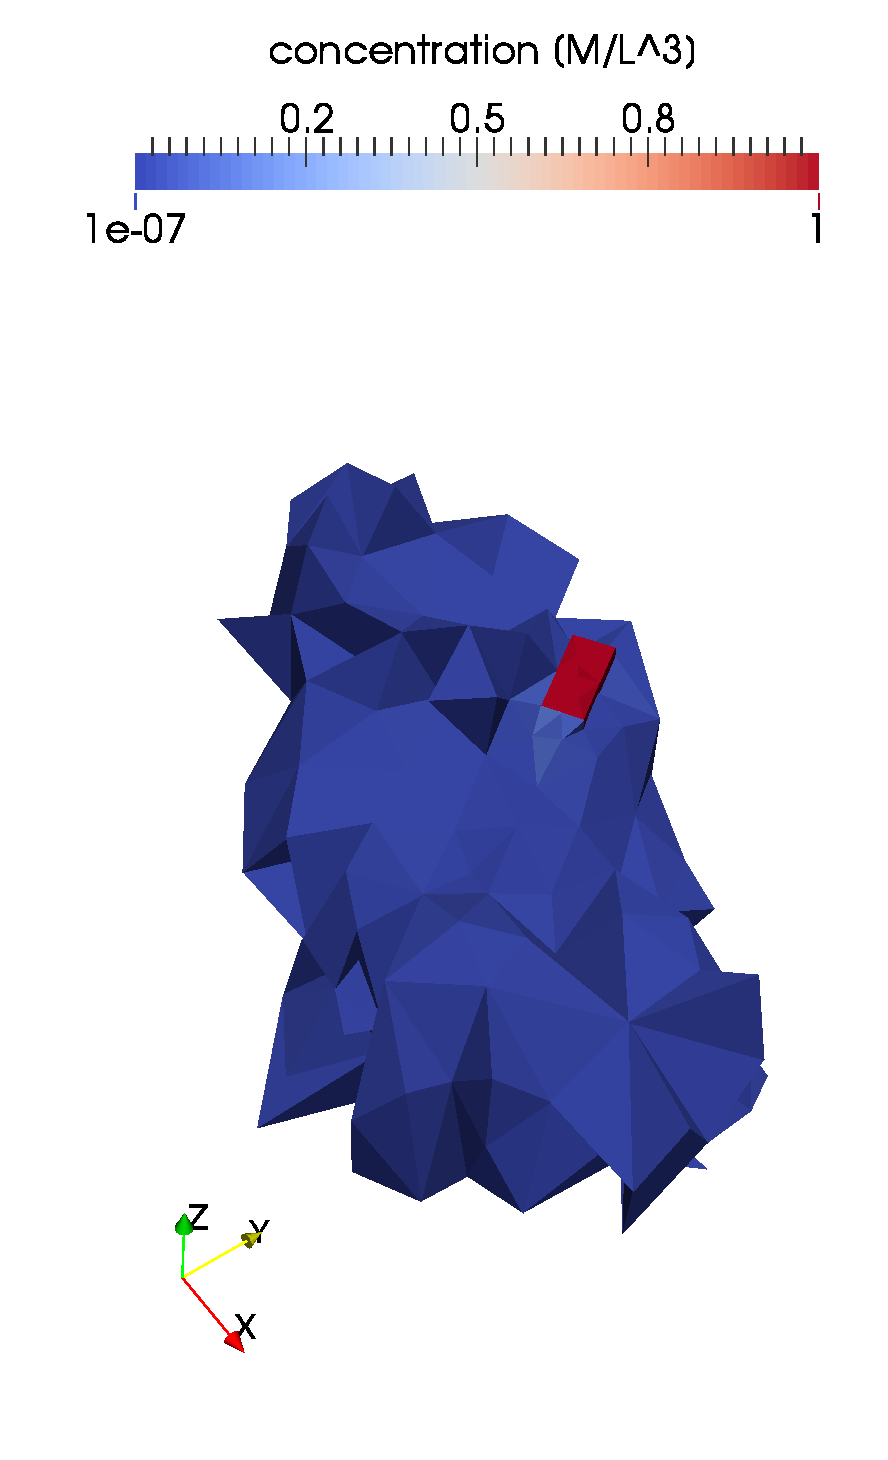
\includegraphics[width=\textwidth]{tests_graphics/transport_end_167o.pdf}
        \caption{Program version 1.6.7, computed with Dirichlet BC.}
        \label{fig:bench_mel3a}
    \end{subfigure}
    ~
    \begin{subfigure}[b]{0.3\textwidth}
        \centering
        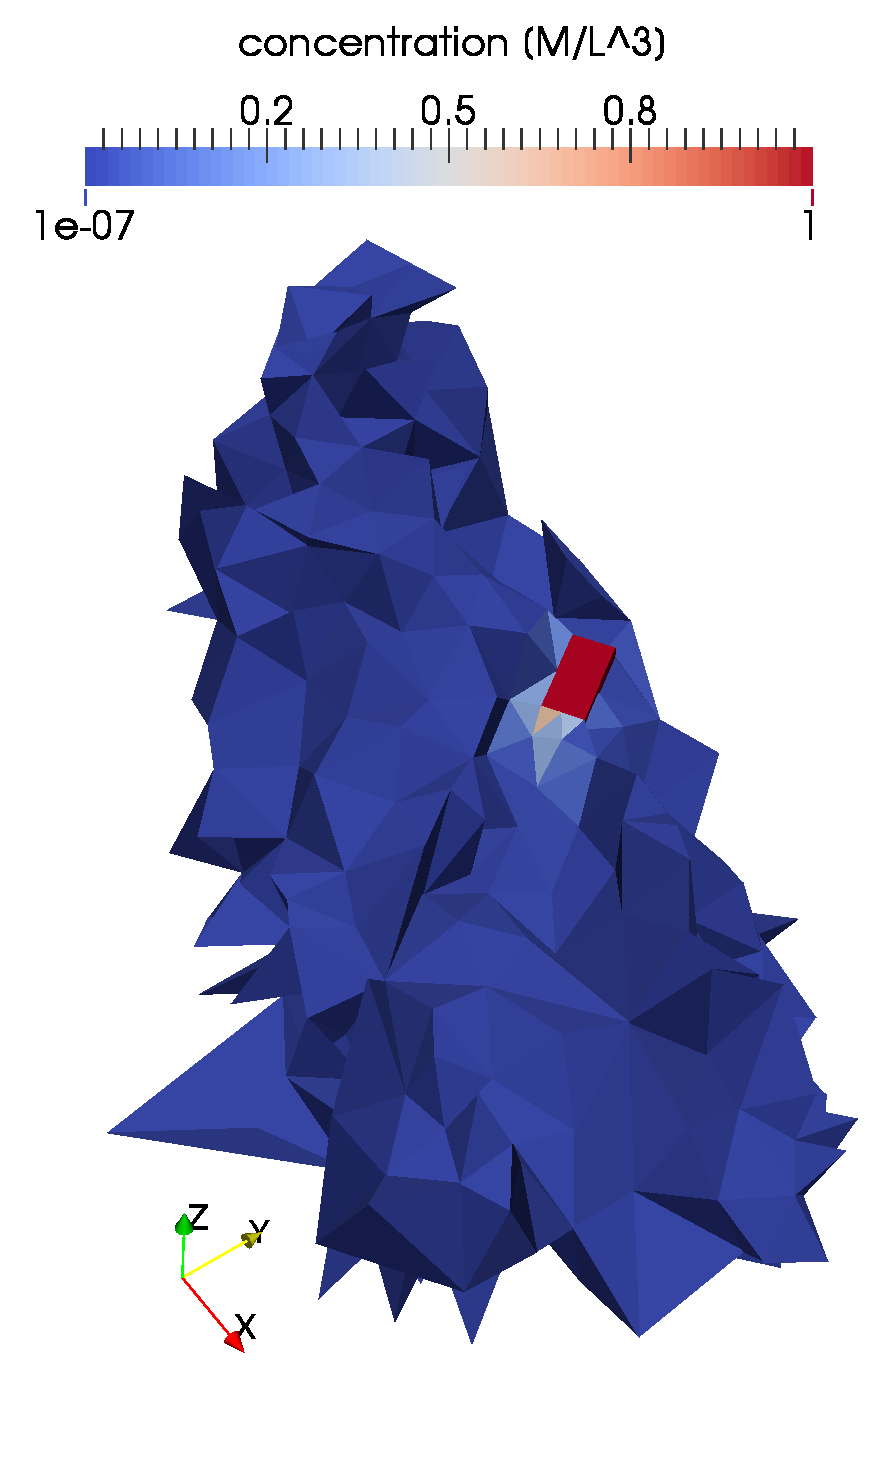
\includegraphics[width=\textwidth]{tests_graphics/transport_end_167s.pdf}
        \caption{Program version 1.6.7, computed with source term prescribed.}
        \label{fig:bench_mel3b}
    \end{subfigure}
    ~
    \begin{subfigure}[b]{0.3\textwidth}
        \centering
        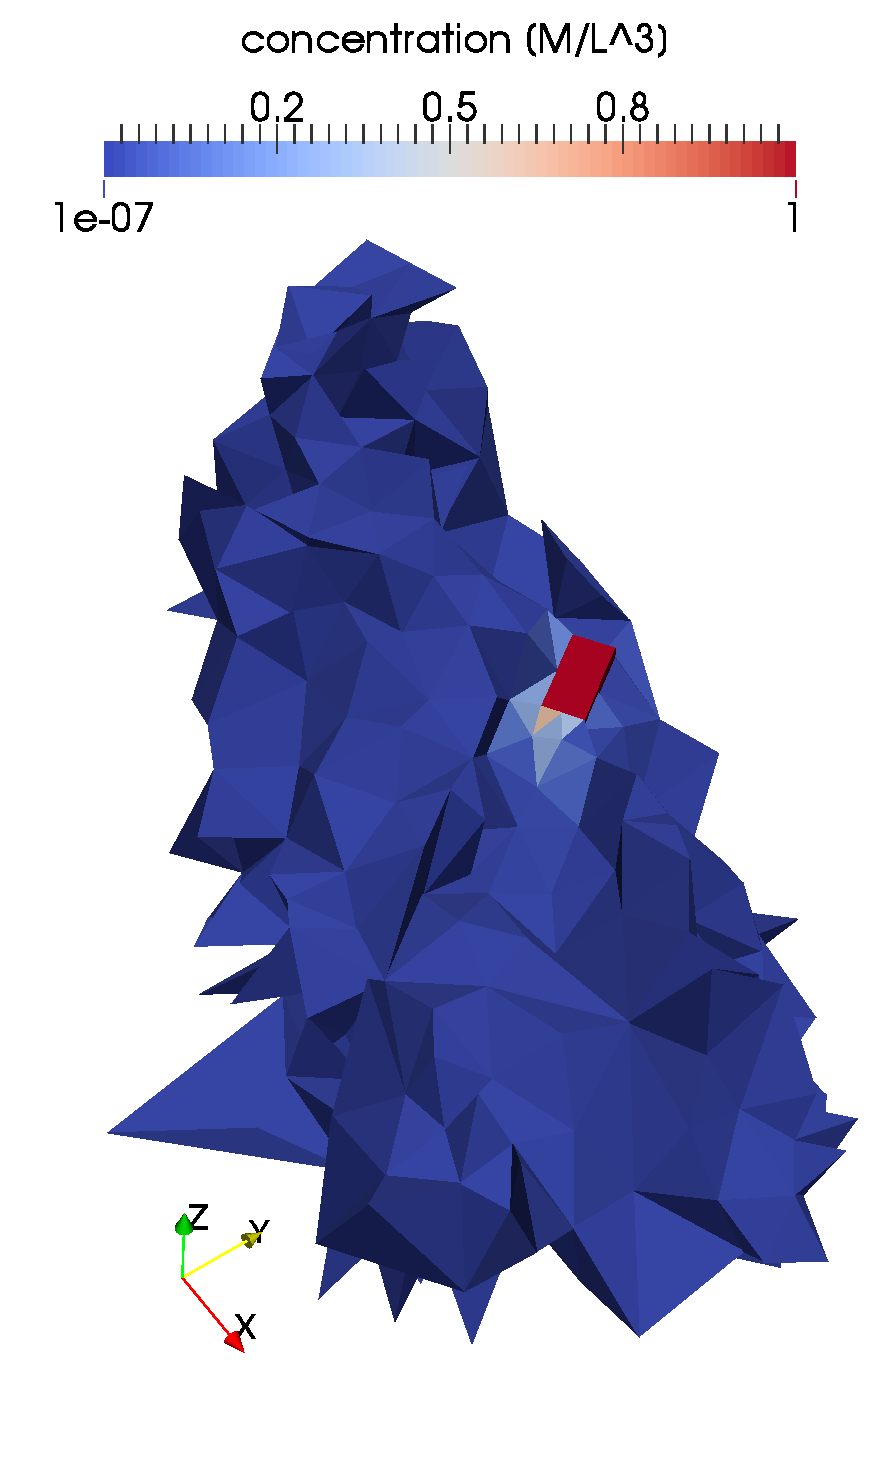
\includegraphics[width=\textwidth]{tests_graphics/transport_end_170.pdf}
        \caption{Program version 1.7.0, computed with source term prescribed.}
        \label{fig:bench_mel3c}
    \end{subfigure}
    \caption{Concentration of the transported substance after $10^5$ years.}
    \label{fig:bench_mel3}
\end{figure}

\textbf{Transport.}
The transport of the substance was computed over time period of $10^5$ years. In the figure \ref{fig:bench_mel3} we can see 
where the substance spread in concentration above $10^{-7}$~\unitss{1}{-3}{} which again corresponds to the solver accuracy.
We can compare the solutions computed by different versions in subfigures \ref{fig:bench_mel3a} to \ref{fig:bench_mel3c}.
The transport is caused only by convection so the velocities computed before are determining. As we can see in the figure 
\ref{fig:bench_mel1}, the difference in velocities is positive which means the velocities were smaller when the Dirichlet 
boundary condition was prescribed on the source region. That is why the convectional transport is also slower in that case 
as we can observe in the figure \ref{fig:bench_mel3a}. 

The transport computed with sources term prescribed is the same in both versions 1.6.7 and 1.7.0 as ilustrated in the figure
\ref{fig:bench_mel3b} and \ref{fig:bench_mel3c}. One can open Paraview state file to see that the difference in transport is in
order $10^{-7}$ corresponding again to the solver accuracy.




\emph{Notice. If user compares the solutions of transport computed in versions 1.6.7 and 1.7.0 in Paraview (or other SW)
be aware of a little bug in version 1.6.7 -- the transport steps are labeled only by numbers (1,2,3,...) not by the 
corresponding times. }


